\documentclass{jarticle}

\usepackage{geometry}
\usepackage{cite}
\usepackage[dvipdfmx]{graphicx}
\usepackage{here}
\usepackage{amsmath}
\usepackage{amsfonts}
\bibliographystyle{junsrt} %参考文献出力スタイル


\geometry{left = 20mm, right = 20mm}
\title{非定常時系列の教師なしクラスタリング:位相的データ解析による分析}
\author{黒木 裕鷹}
\date{2018年4月27日}

\begin{document}
\maketitle
\section{はじめに}
膨大な特徴量をもつ高次元データ解析において,どのように高次元の特徴量を低次元で表現するのかは重要な研究課題である.近年,位相的データ解析による高次元データ解析が盛んに提案されており,複雑な高次元データの位相的情報を可視化する手法として注目を集めている.

位相的データ解析では、主としてパーシステントホモロジー\cite{Edelsbrunner2002}という、ホモロジーの誕生と消滅に着目することにより、データの位相的情報を抽出する手法が用いられる。
このパーシステントホモロジーを可視化したパーシステントダイアグラム\cite{Otter2017}を解析することによる知識発見や、変数間のネットワーク構造の解明に役立つことが期待されている。

位相的データ解析を利用した研究としては、複数方向からのシルエット画像からパーシステントホモロジーを構成し歩行識別を行った\cite{Lamar2012}、\cite{Platt2016}による病気に寄与する遺伝子の解析、\cite{Gidea2017}による金融危機の早期察知,\cite{Gidea2018}による金融資産間の相関構造の推移に関する分析などがあり、その応用分野は多岐にわたる。

現在,世界の様々な工場では産業用ロボットが用いられている.
産業用ロボットの導入の目的は、人間には負担の大きい作業の代替のためであり、例えば、重量物の運搬や作業場に霧散している粉塵の吸入にリスク回避等を目的としている。
産業用ロボットはこのような安全性の問題を解決するだけでなく,単純作業の代替などによる人件費削減など、経済性や効率性においてもメリットがある.
一方、ロボットには故障のリスクがあり,ただひとつのロボットの故障が生産ライン全体に影響を及ぼし得る.
故障を未然に回避するためにはメンテナンスなどの保守作業を行うことが重要であるが,メンテナンスや部品交換にも費用や時間などコストがかかるため,適切なタイミングで行われることが望ましい.


自動車メーカーのMでは,生産ラインで使用するアームロボットの故障を未然に防ぐため,その減速機の交換を経験に基づくタイミングで行っている.
交換のタイミングが遅すぎれば故障を招くが,早すぎても交換に時間がかかる分パフォーマンスが低下することとなる.
本調査では,ロボットアームをモニタリングした振動のセンサーデータを用い,減速機交換前後のデータに明確な違いがあるかどうかを調査した.
ロボットの故障により生産ラインを止めることはあってはならないため,故障直前のデータは得ることが出来ないことに留意しなければならず,教師無し学習によるクラスタリングを行うことを目的とした.


Mより提供されたデータは一つのロボットアームにつき,減速機交換前後それぞれで5秒間の計測を10回行った1次元の振動データである.
ロボットアームはそれぞれ挙動が異なるため,その主要な振動はアームごとに異なっている.
また,各アームの行動1セットは5秒間ではないため,各計測ごとにより行動セットの中の計測する部分が異なっている.

複数のロボットアームの振動は高次元時系列として与えられる。
また、各アームやセンサー取り付け位置に応じて、振動パターンの形状は様々な周期的変動パターンを持つ。
ことのうな非定常高次元高頻度時系列のクラスタリングに対する統一的な統計分析手法は存在しない。
多変量解析における階層的クラスタ分析では、クラスタリングされる対象間の類似度もしくは非類似度が必要である.
時系列を対象としたクラスタリングにおいて,最も広く使用されている非類似度はユークリッド距離,Dynamic Time Warping(DTW)\cite{Berndt1996},CORT\cite{Chouakria2007}などである.
スペクトル密度関数を特徴とするクラスタリングは、などによって提案されている。
DTWは2つの時系列データの異なる2時点間全ての誤差を計算し,一定の制約の元でそれらの合計が最小になるような一致を求めるアルゴリズムである.
DWTやCORTによる分析は、例えば、、や。。の分析を対象に行われ、、、などの有用性が示されている。
DWTを用いることのメリットは、DTWは二つの時系列の周期や長さが異なる場合でも非類似度を算出することができることが挙げられる.
DTWにより挙動の計測開始時点が異なる問題は多少解決されるが,振動の形状の大部分はロボットアームの挙動によって異なるため,減速機交換前後の差異はクラスタリングの結果に表れない.
また,未知音源分離などで用いられるFastICA\cite{Hyvarinen2000}などの独立成分分析(ICA)のアルゴリズムは、主要な振動と微細な振動を分けることを可能にするかもしれない。
しかし,同時点の複数観測を必要とする他、未知音源の数を指定する必要があり、本データには適用することはできない.
時系列の同時性を利用することなく,かつアームごとに異なる主要な振動に影響されない特徴量によって教師無し学習を行うことが課題である.
本調査では,以上のような課題を解決するため,データの位相的な特徴に注目した.
データの位相的特長を分析することにより、故障につながり得るロボットアームの劣化を抽出することを目的とする。

近年着目されているTopological Data Analysis(TDA)は複雑なデータを扱う上で強力であり,パーシステント・ホモロジー\cite{Edelsbrunner2002}とその表現であるパーシステントダイアグラム\cite{Otter2017}をはじめとするその手法はデータの位相的特徴を抽出し,新しい知見を与える.
またTDAの分野で広く行われているように,時間遅れ座標を用いて時系列を多次元に埋め込むことで位相的特徴を抽出する足掛かりとした.
時間遅れ座標による埋め込みはダイナミカルシステムの分野で,状態空間の復元を目的に広く用いられている.
パーシステント・ダイアグラムを比較するためにWasserstein距離\cite{Mileyko2011}がしばしば用いられるが,本調査で扱うような高頻度データでは計算量の観点で現実的ではない.
また,\cite{Umeda2017}の提案するBetti sequenceはデータの位相情報を1次元の系列として要約する.
そこで本調査では,観測の上述した観測の長さや観測開始時点が異なる問題を解決するためにセンサーデータの位相情報を要約したBetti sequenceをもとめ,DTWに基づく全結合型階層的クラスタリングを行うことにより,減速機交換前後の振動を分析した.


本レポートの構成は次のようである.
まず2節では本調査で使用したTDAの手法やクラスタリング手法について述べ,3節では実際のデータ解析とその結果を示す.
4節では考察を行うと共に今後の展望について触れる.

\section{Topological Data Analysis(TDA) と時系列クラスタリング}
位相空間とは、集合に距離関数を定義することなく、直接開集合となる部分集合を定めてできる空間である。
位相的データ解析では、距離関数に縛られないやわらかい幾何情報を扱い、データの情報を抽出する。
その主要な手法はmapper\cite{Singh2007}とパーシステント・ホモロジー\cite{Edelsbrunner2002}である.
これらはノイズを含む複雑なデータセットから何か新たな知見を得る目的でしばしば用いられてきた.
本調査ではパーシステント・ホモロジーを利用する.

\subsection{パーシステント・ホモロジー}
ユークリッド空間の有限点集合を$X$,点$x_i \in X$を中心とした半径$r$の球の和集合を$B(X;r):=\bigcup_{i=1}^n B(x_i;r)$とする.
ただし,$B(x;r) =\{y \in M | d(x,y) \leq r\}$($d(x,y)$は$x,y$のユークリッド距離)とする.
球の和集合を半径パラメータ$r$で集めた集合$\mathbb B(X):=\{B(X;r)\}_{r\geq 0}$をここでは$X$のフィルトレーションという.
$r\leq a$ならば包含関係$B(X;r)\subset B(X;a)$があるため,ホモロジー群間の射$u_r^a : H_q(B(X;r))\rightarrow H_q(B(X;a)) $を包含写像から誘導する.
このとき,ホモロジー群の系列
$$
H_q(\mathbb B(X)):\dots\rightarrow H_q(B(X;r))\overset{u_a^b}{\rightarrow} H_q(B(X;a))\rightarrow\dots (r\leq a)
$$
を$X$の$q$次元パーシステントホモロジーという.
また、パーシステントホモロジーは分解定理\cite{Zomorodian2005}により、適切な区間表現$\mathbb I[b_i, d_i] $を通じて
$$
H_q(\mathbb B(X))\cong\oplus I[b_j,d_j] (b_j\leq d_j)
$$
で一意に表現される.ここで、区間$I[b_j,d_j]$はq次ホモロジー$j(j=1,\dots,J_q)$が発生($b_j$)してから消滅($d_j$)するまでの$r$の区間である。これをユークリッド空間$\mathbf R^2$内にプロットした散布図
$$
D_q(X):= \{(b_j,d_j) | j \in J_q\}
$$
を$X$の$q$次元パーシステント・ダイアグラムという.
パーシステント・ダイアグラムの元$(b_j, d_j)$はホモロジーの生成元の発生時間(Birth time)を$b_j$,消滅時間(Death time)を$d_j$と記録しているものと解釈できる.

$q$次のパーシステント・ダイアグラムは2次元の散布図として表され,その解釈や扱いが困難である.
そのため,様々なダイアグラムの要約が提案されてきた.
最も単純な要約が最大パーシステンスであり,$\text{max}_j(b_j - d_j)$
で表され、最も特徴的なホモロジーの持続性を表意味する。


\subsection{パーシステント・バーコード}
前節で定義したダイアグラム$D_q(X)$のホモロジー$j$に対して,次の$s_j(r)$を定義する.
$$
s_j(r) = 
\begin{cases}
1 & (b_j \leq r \leq d_j)\\
0 & otherwise
\end{cases}
$$
$s_j(r)$を並べてプロットしたものをパーシステント・バーコードという.

また,\cite{Umeda2017}はバーコードを単純に扱い,機械学習の枠組みで扱いやすくするために次で提案されるBetti sequence,$BS(X)$を提案している.
$$
BS(X) = \sum_j s_j(r)
$$
Betti sequenceは半径$r$のときにいくつのホモロジーが存在しているかを表す1次元の系列となる.

\subsection{1次元時系列データに対するTDA}
時系列から複数次元の有限点集合を構成する方法として,遅れ時間座標を利用した埋め込み(embedding)がある.
埋め込みはアトラクタを再構成するために非線形ダイナミカルシステムの分野で盛んに利用されている.
長さ$N$の時系列$x_1, x_2, \dots , x_T$から適当な遅れ時間$\tau$ごとの$d$個の測定値を取り出し$V(t) = (x(t), x(t+\tau), \dots, x(t + d - 1)),\ (t = 1,2,\dots, T)$の$d$次元有限点集合を得る.
この有限点集合が元の$k$次元力学系の埋め込みになるための十分条件として,$d\geq 2k+1$(ターケンスの埋め込み定理\cite{Takens1981})が知られている.

また,有限点集合の次元$d$が大きくなったときに$\mathbb R^d$の$n$個の点集合のドロネー三角形分割の計算量は$\mathcal O(n^{\frac{[d]}{2}})$になりうる\cite{Amenta2007}, \cite{Attali2003}.
そこで,位相情報を保持しながら計算を簡略化するため,十分多次元に埋め込んだ後主成分分析により3次元に次元削減するアプローチが提案されている\cite{Truong2017}.


\subsection{時系列クラスタリング}
時系列間の非類似度を算出する際,用いられているのが\cite{Berndt1996}で提案されたDynamic Time Warping(DTW)である.
DTWは三角不等式を満たさないため距離ではないが,比較的少ない計算量で要素数の異なる系列同士の距離のような量を求める手法である.

また本調査ではDTWに基づき,完全連結方による階層型クラスタリングを行った.
完全連結法とは,クラスタ間で最も類似度が低いデータ間の距離をクラスタ間の距離にする方法である.







\section{データ解析}

\subsection{データの概観}
本調査では,自動車メーカーMの産業用ロボットアームの振動データを扱う.
15種類のロボットアームに対し,減速機を交換する前と交換した後をそれぞれ10回モニタリングした合計300系列のデータである.
計測の基本単位は100ミリ秒であり,計測の長さは5秒間である.ロボットアーム15種類の減速機交換前後のデータのそれぞれ10回分の観測を連結し,以下の図\ref{fig:ts}にプロットした.
このように,いずれのロボットアームにおいてもその時系列は明らか非線形構造を持つと同時に交換前後の系列の挙動は類似しておりは,アームごとに特有の周期的な振動を持つことがわかる.
減速機交換前後の特徴を目視で判断することはできない.
さらに交換前後で計測開始時間が異なるものもあり,単純な比較が難しいことがわかる.
\begin{figure}[htbp]
\begin{center}
	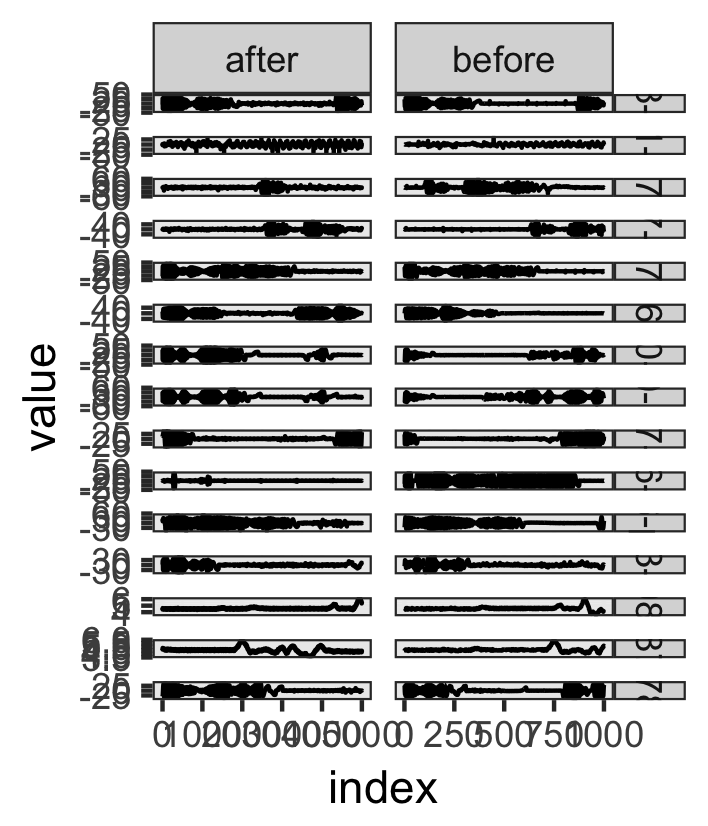
\includegraphics[width=12cm]{fig/ts.png}	
	\caption{センサーデータの時系列プロット\label{fig:ts}}
\end{center}
\end{figure}

\subsection{データの位相的特徴}
ロボットアームによる振動のスケールを調整するため,以下の分析は予め全系列を標準化した上で行った.
1次元の振動時系列から位相情報を取り出すために,遅れ時間座標への埋め込みを行った.
その際,遅れ時間単位は$\tau = 1$とした.
またロボットアームの構造や状態変数の数が明らかでないことから,埋め込み次元にはロボットアームが3次元であることを考慮し,ターケンスの埋め込み定理\cite{Takens1981}を参考に$d = 3\times2 + 1 = 7$とした.
さらに\cite{Truong2017}で提案されているように主成分分析を用い第3主成分までを取り出し3次元の有限点集合を抽出した.
アルファ複体のフィルトレーションを用いて抽出した点集合の$0,1,2$次元パーシステントホモロジーを計算した.
0次のホモロジーは連結を、1次は穴を、2次は空洞であるので、それぞれのパーシステントホモロジーはその発生と消失を表す。
またその要約として各次元のBetti sequenceを計算し,以下の図\ref{fig:betti1}, \ref{fig:betti2}に示した

\begin{figure}[htbp]
\begin{center}
	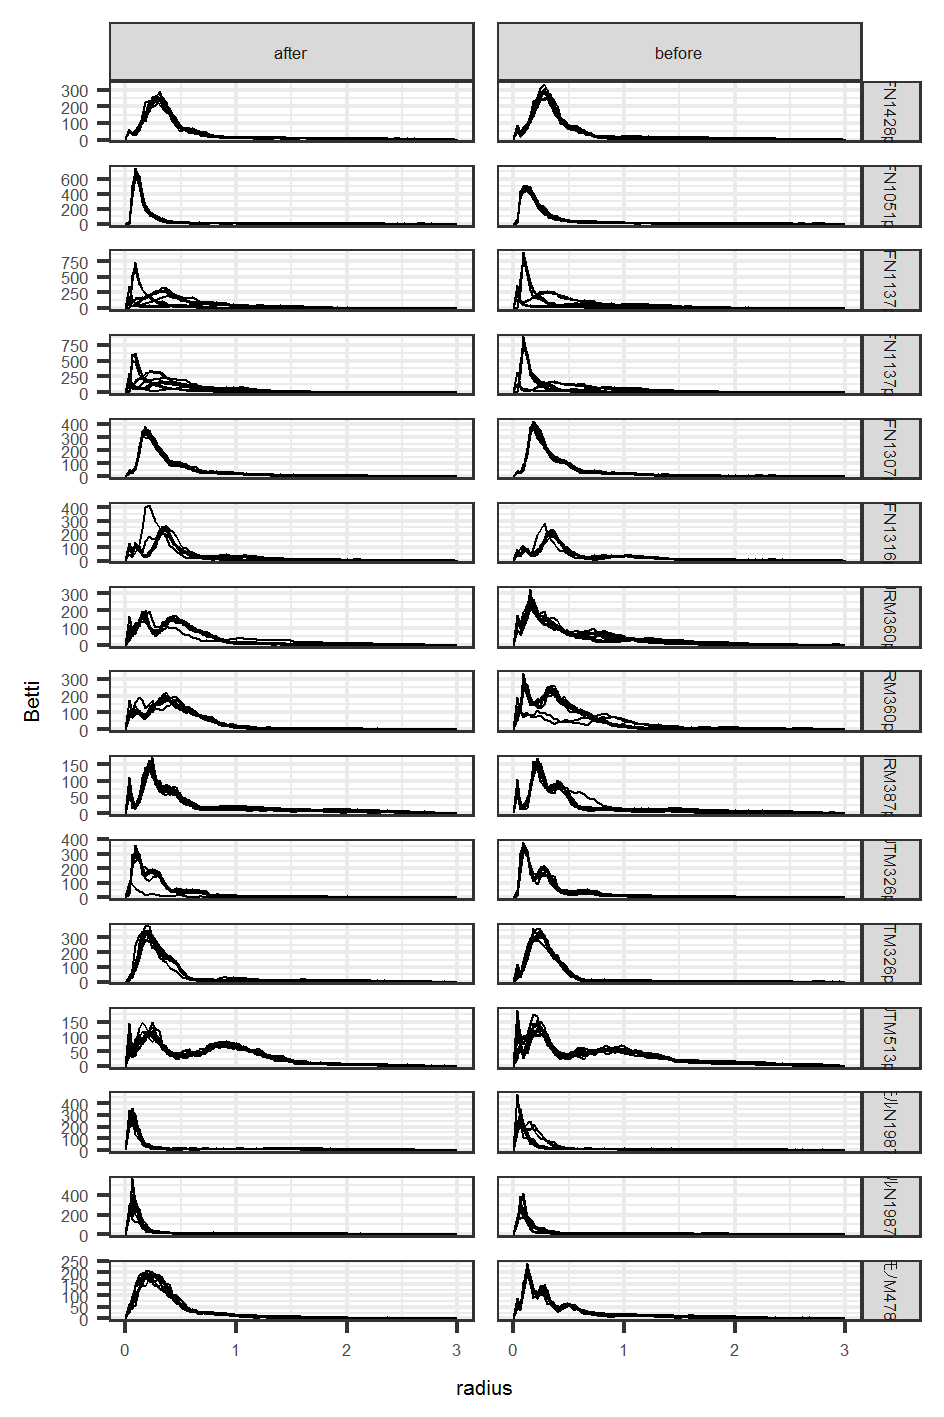
\includegraphics[width=11cm]{fig/betti_1.png}	
	\caption{1次のBetti sequence}\label{fig:betti1}
\end{center}
\end{figure}

\begin{figure}[htbp]
\begin{center}
	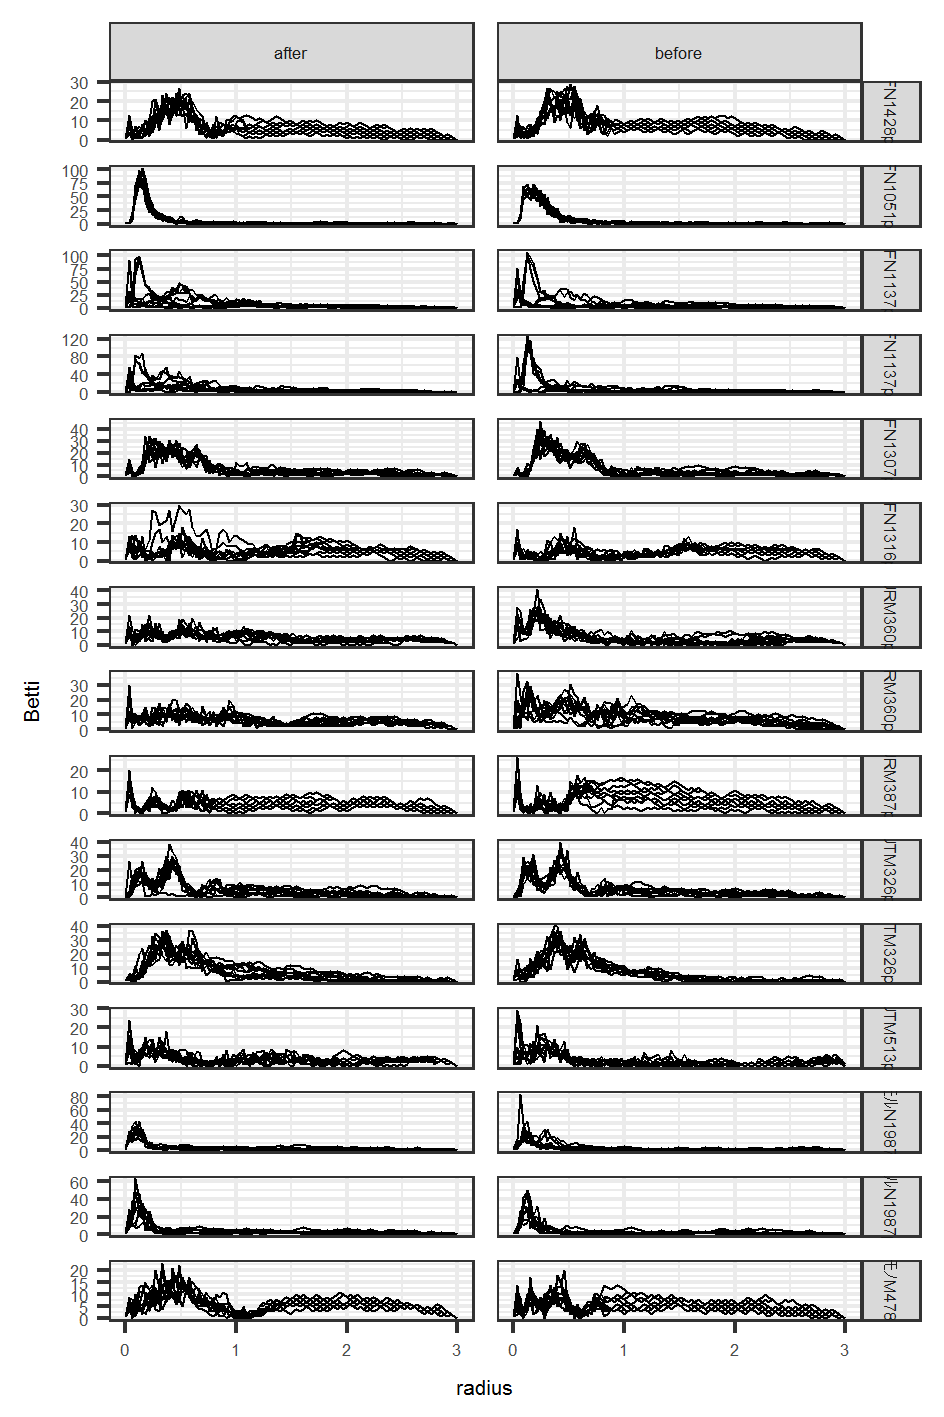
\includegraphics[width=11cm]{fig/betti_2.png}	
	\caption{2次のBetti sequence}\label{fig:betti2}
\end{center}
\end{figure}

Betti sequenceは、その時(半径)にいくつのホモロジーが存在しているのかを表すのであった。
図\ref{fig:betti1}, \ref{fig:betti2}より,ロボットアームごとにホモロジーの数の推移が異なり、位相的特徴が抽出されている。
また,2次のBetti sequenceは1次のものに比べて観測ごとのばらつきが大きくなっていることが見て取れる.
観測ごとのノイズに影響を受けている可能性があり、2次のBetti sequenceについては扱いに注意が必要である。
しかし、ロボットアームごとにその概形が異なることから、位相的特徴は抽出されている。

\subsection{DWTに基づいた時系列クラスタリング}

ロボットアームごとに減速機交換前10系列,交換後10系列の計20系列をクラスタリングする.
観測ごとのばらつきが少ない1次のベッチ数をもとにDTWを比類似度とした階層的クラスタリングを行った.
クラスター間の距離は完全連結法を用いて算出した.
そのデンドログラムを図\ref{fig:dendro1}から図\ref{fig:dendro15}に示した.

図\ref{fig:dendro1}から図\ref{fig:dendro15}より,いくつかのロボットアームでは明確に減速機交換前後のクラスタが構成できたことが分かる.
またそうでないアームでも細かい部分では減速機交換前後のクラスタができていることが分かる.

\begin{figure}[H]
	\begin{center}
		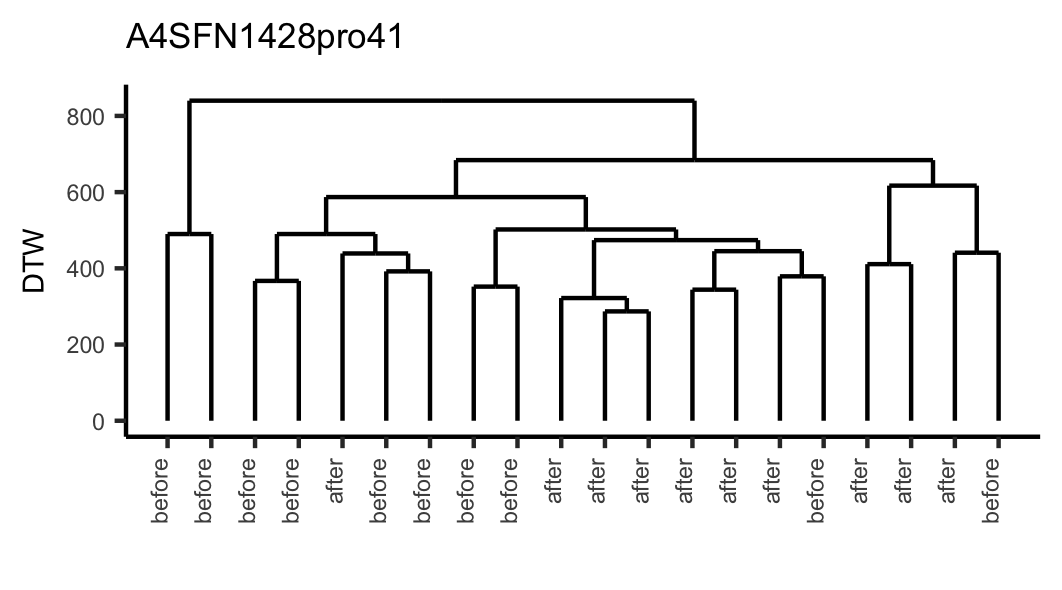
\includegraphics[width=15cm]{fig/dendro_1.png}
		\caption{デンドログラム1}
		\label{fig:dendro1}
	\end{center}
\end{figure}
\begin{figure}[H]
	\begin{center}
		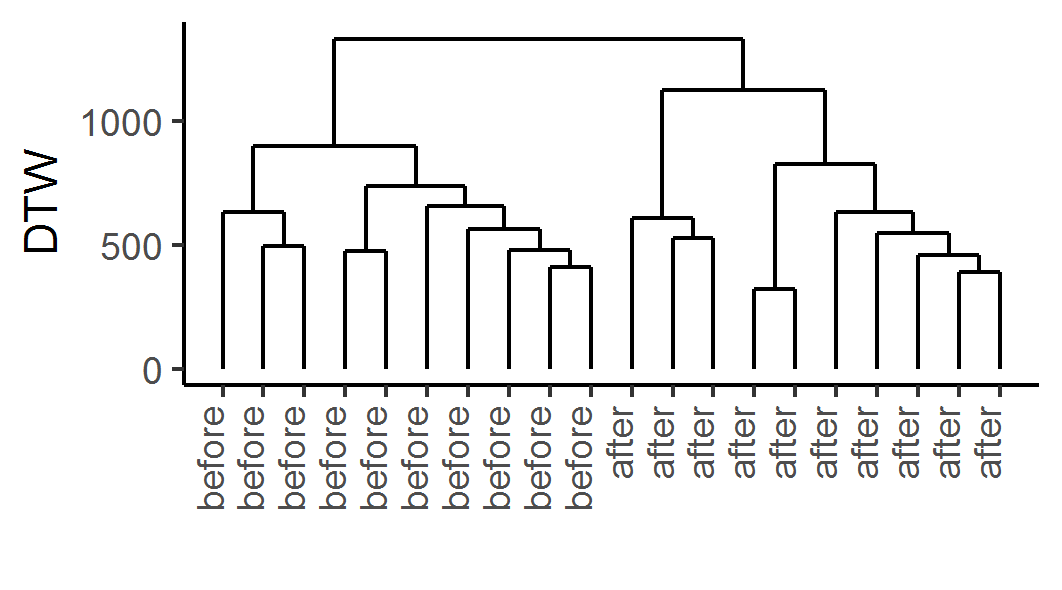
\includegraphics[width=15cm]{fig/dendro_2.png}
		\caption{デンドログラム2}
		\label{fig:dendro2}
	\end{center}
\end{figure}
\begin{figure}[H]
	\begin{center}
		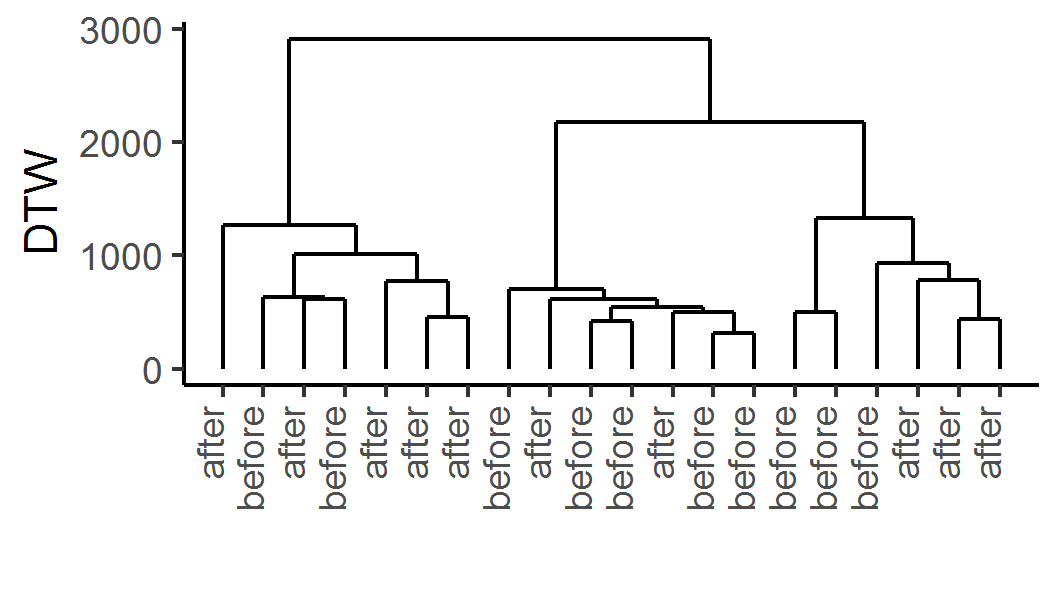
\includegraphics[width=15cm]{fig/dendro_3.png}
		\caption{デンドログラム3}
		\label{fig:dendro3}
	\end{center}
\end{figure}
\begin{figure}[H]
	\begin{center}
		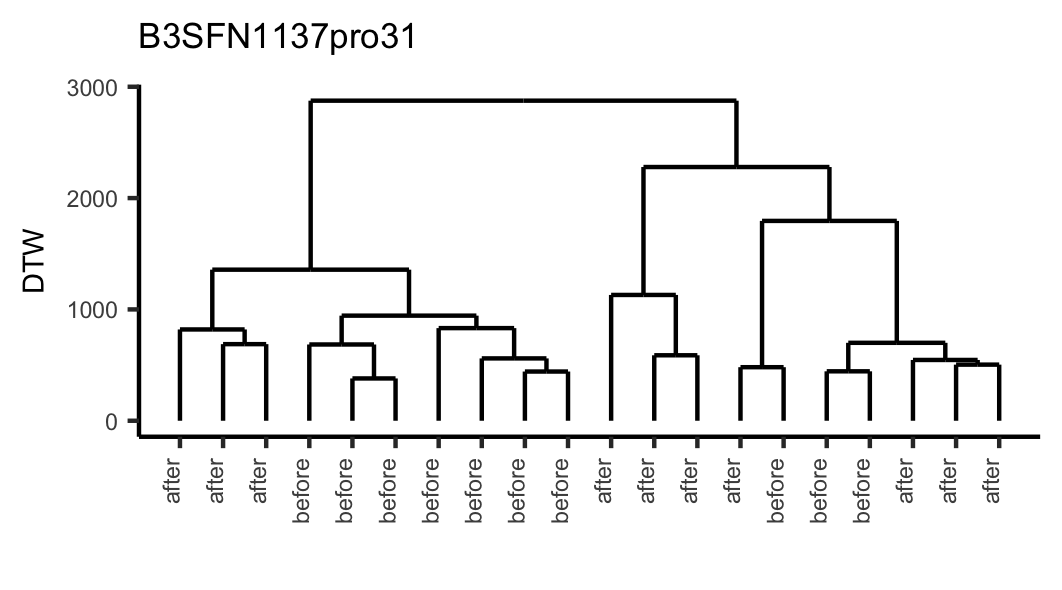
\includegraphics[width=15cm]{fig/dendro_4.png}
		\caption{デンドログラム4}
		\label{fig:dendro4}
	\end{center}
\end{figure}
\begin{figure}[H]
	\begin{center}
		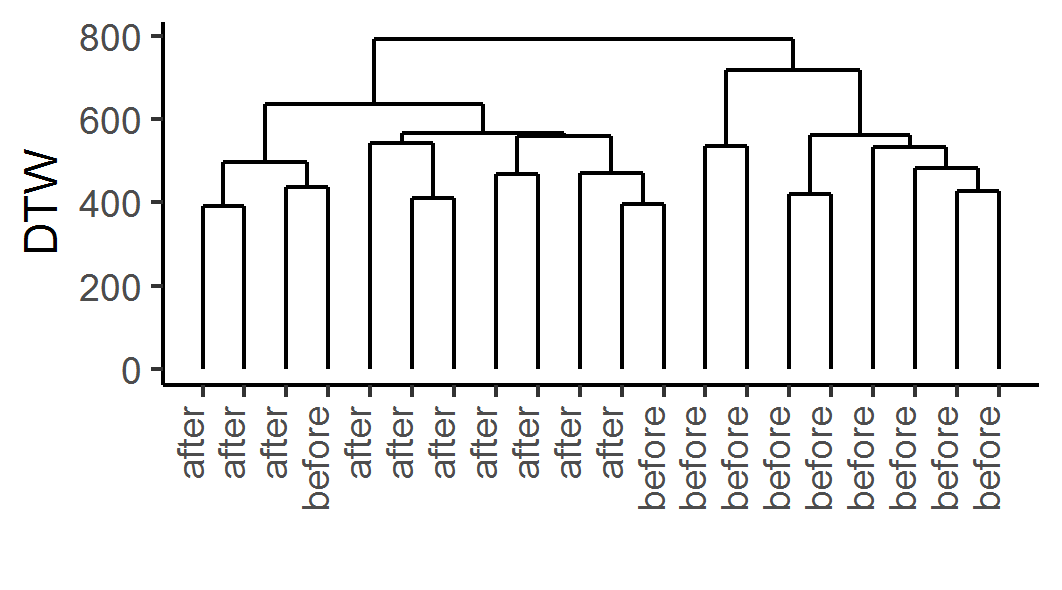
\includegraphics[width=15cm]{fig/dendro_5.png}
		\caption{デンドログラム5}
		\label{fig:dendro5}
	\end{center}
\end{figure}
\begin{figure}[H]
	\begin{center}
		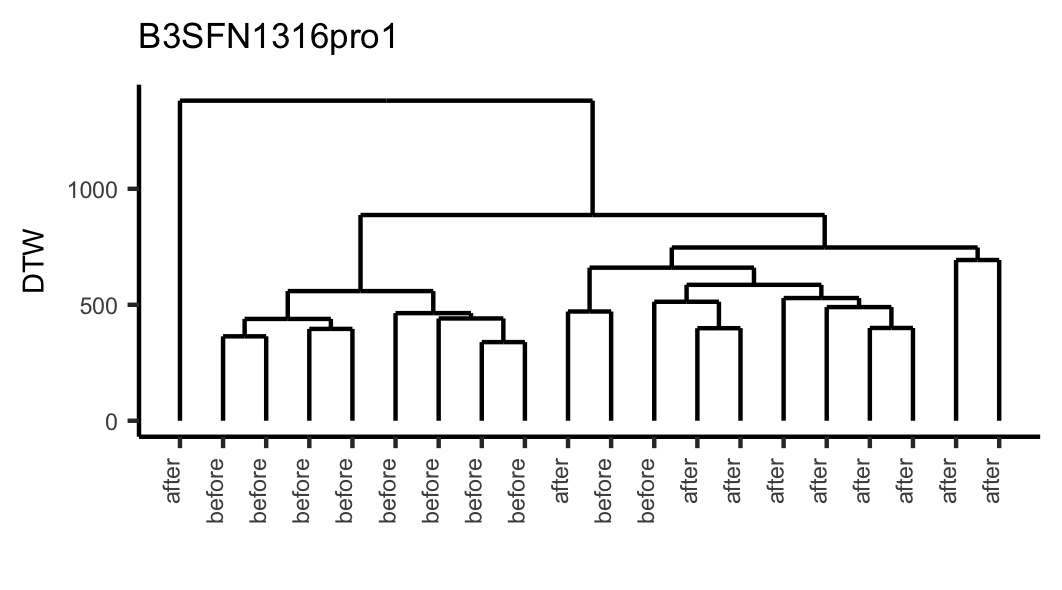
\includegraphics[width=15cm]{fig/dendro_6.png}
		\caption{デンドログラム6}
		\label{fig:dendro6}
	\end{center}
\end{figure}
\begin{figure}[H]
	\begin{center}
		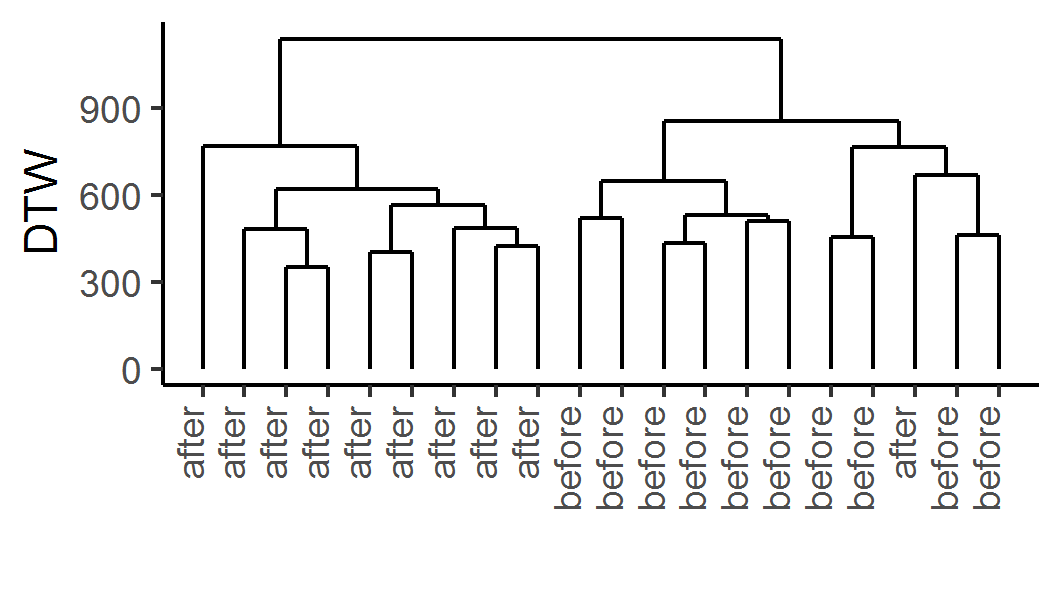
\includegraphics[width=15cm]{fig/dendro_7.png}
		\caption{デンドログラム7}
		\label{fig:dendro7}
	\end{center}
\end{figure}
\begin{figure}[H]
	\begin{center}
		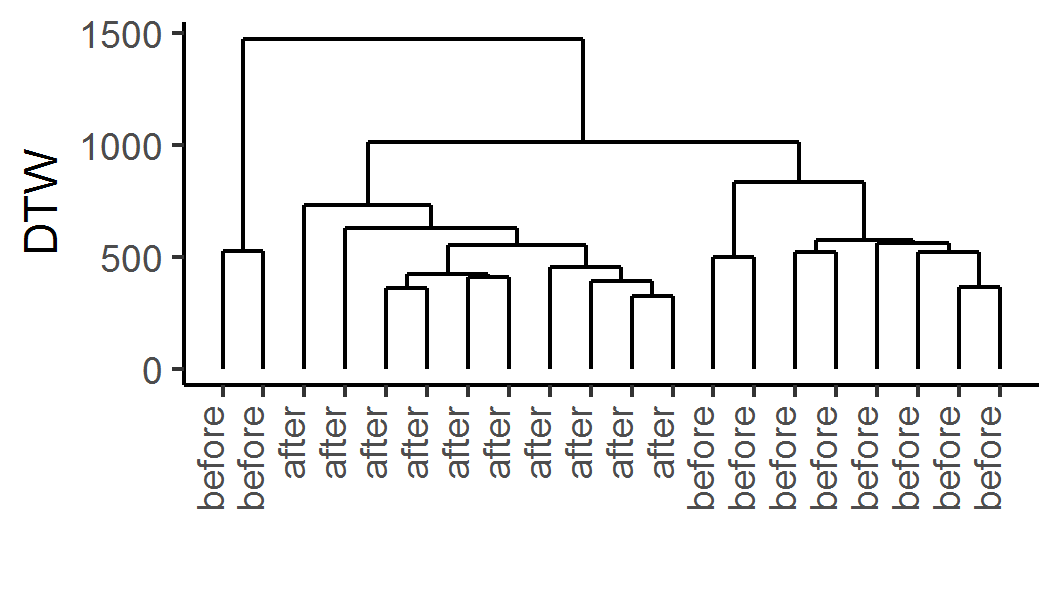
\includegraphics[width=15cm]{fig/dendro_8.png}
		\caption{デンドログラム8}
		\label{fig:dendro8}
	\end{center}
\end{figure}
\begin{figure}[H]
	\begin{center}
		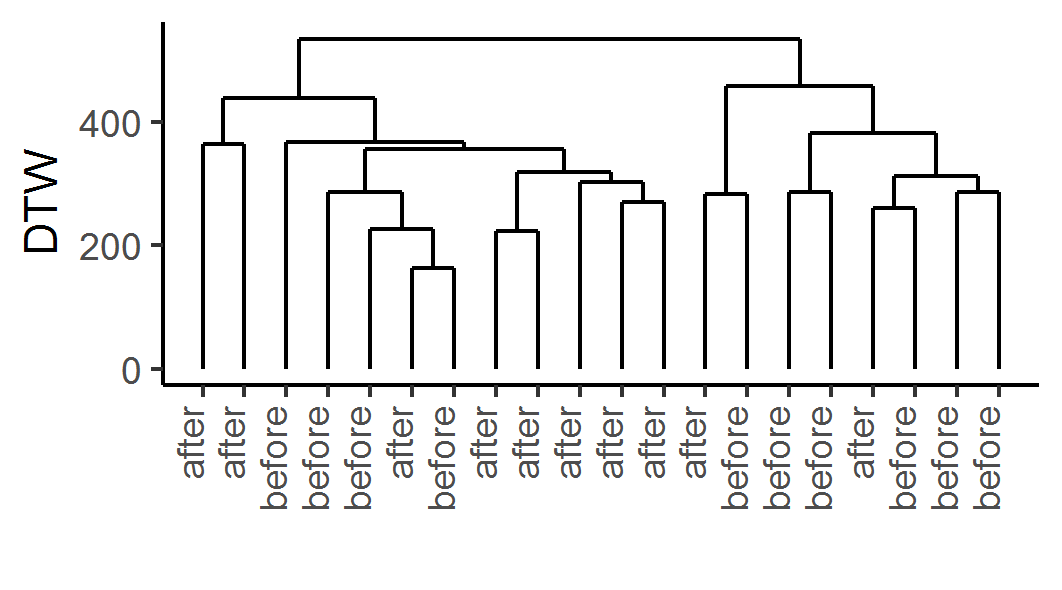
\includegraphics[width=15cm]{fig/dendro_9.png}
		\caption{デンドログラム9}
		\label{fig:dendro9}
	\end{center}
\end{figure}
\begin{figure}[H]
	\begin{center}
		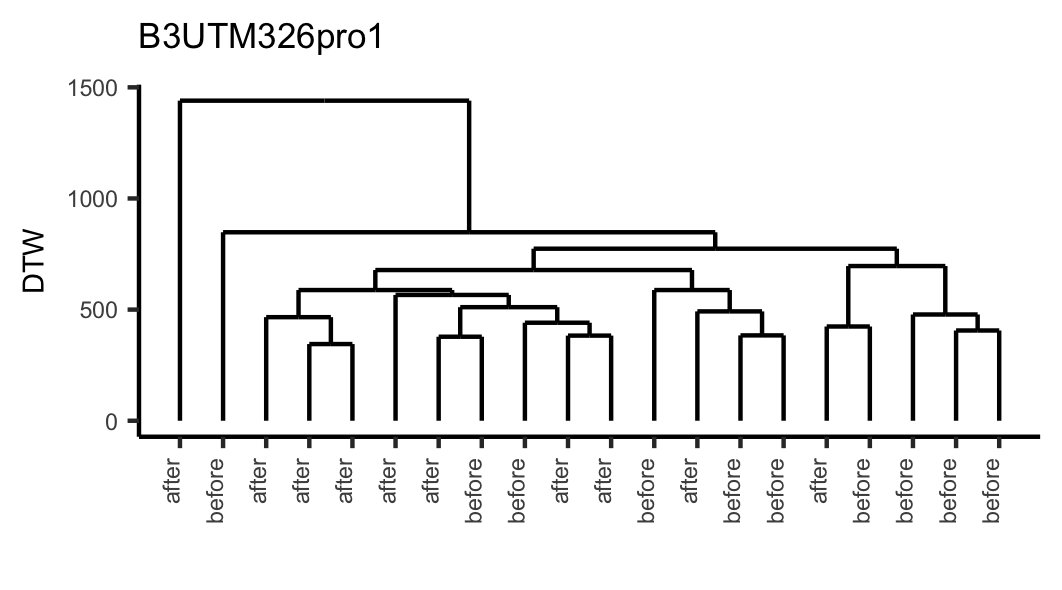
\includegraphics[width=15cm]{fig/dendro_10.png}
		\caption{デンドログラム10}
		\label{fig:dendro10}
	\end{center}
\end{figure}
\begin{figure}[H]
	\begin{center}
		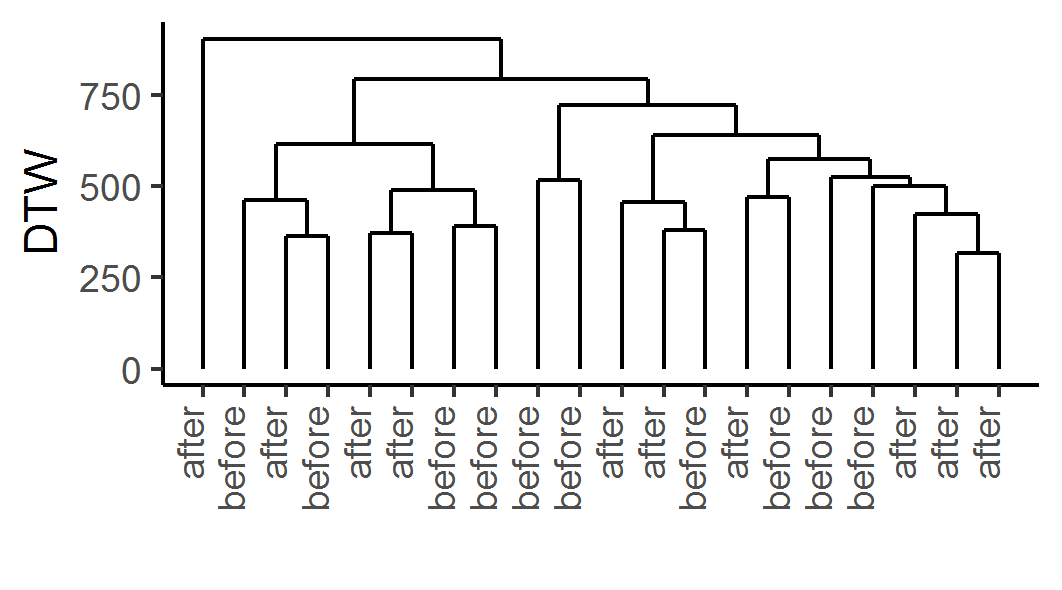
\includegraphics[width=15cm]{fig/dendro_11.png}
		\caption{デンドログラム11}
		\label{fig:dendro11}
	\end{center}
\end{figure}
\begin{figure}[H]
	\begin{center}
		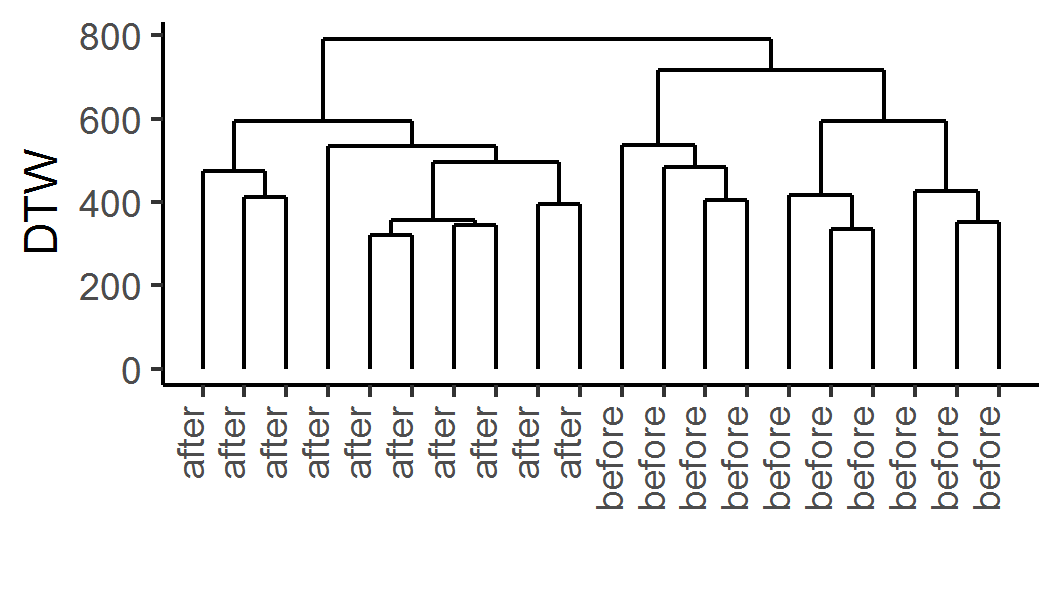
\includegraphics[width=15cm]{fig/dendro_12.png}
		\caption{デンドログラム12}
		\label{fig:dendro12}
	\end{center}
\end{figure}
\begin{figure}[H]
	\begin{center}
		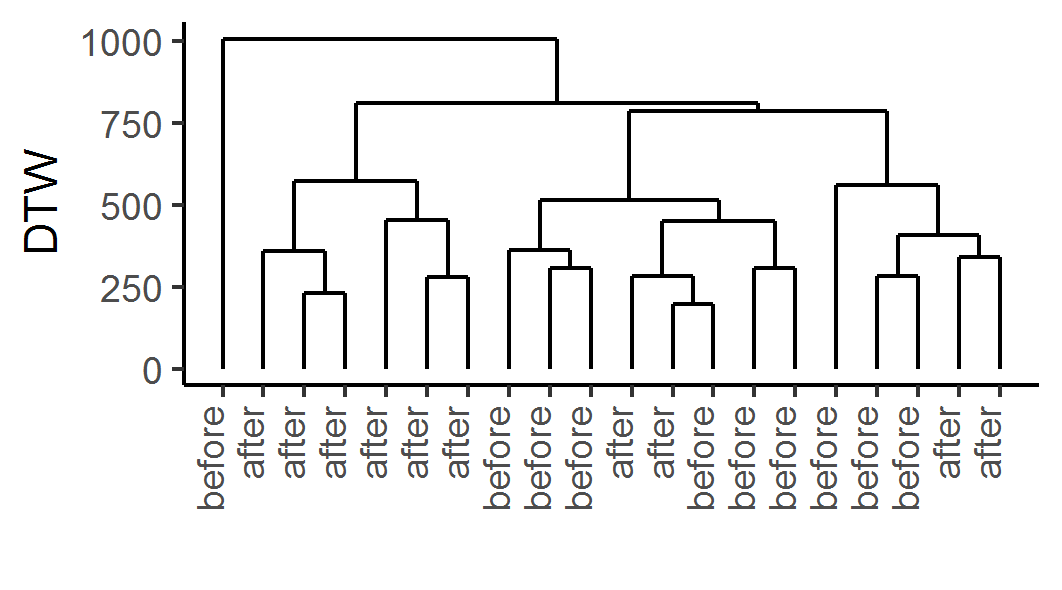
\includegraphics[width=15cm]{fig/dendro_13.png}
		\caption{デンドログラム13}
		\label{fig:dendro13}
	\end{center}
\end{figure}
\begin{figure}[H]
	\begin{center}
		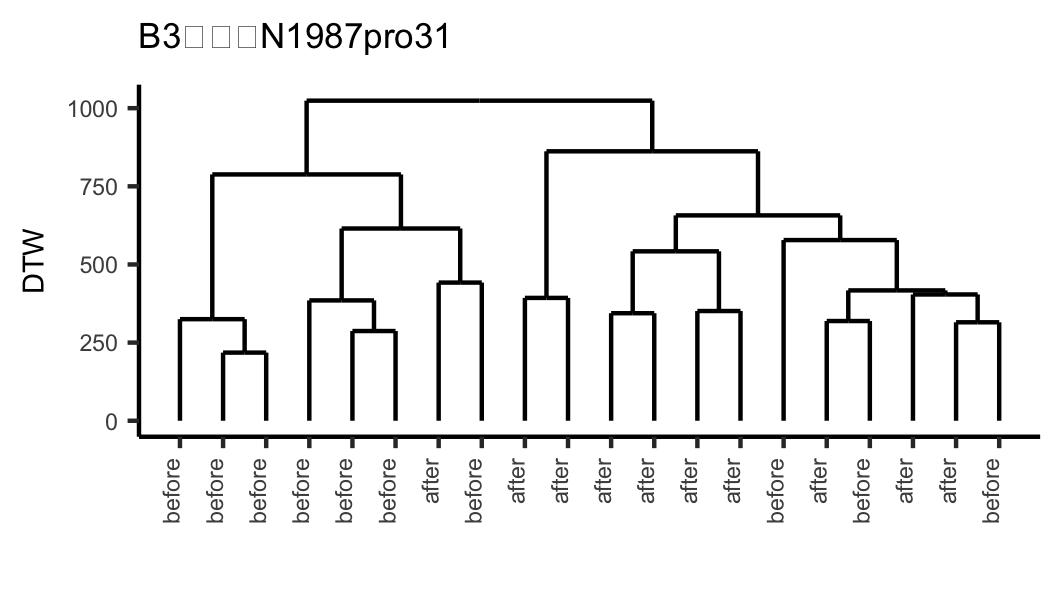
\includegraphics[width=15cm]{fig/dendro_14.png}
		\caption{デンドログラム14}
		\label{fig:dendro14}
	\end{center}
\end{figure}
\begin{figure}[H]
	\begin{center}
		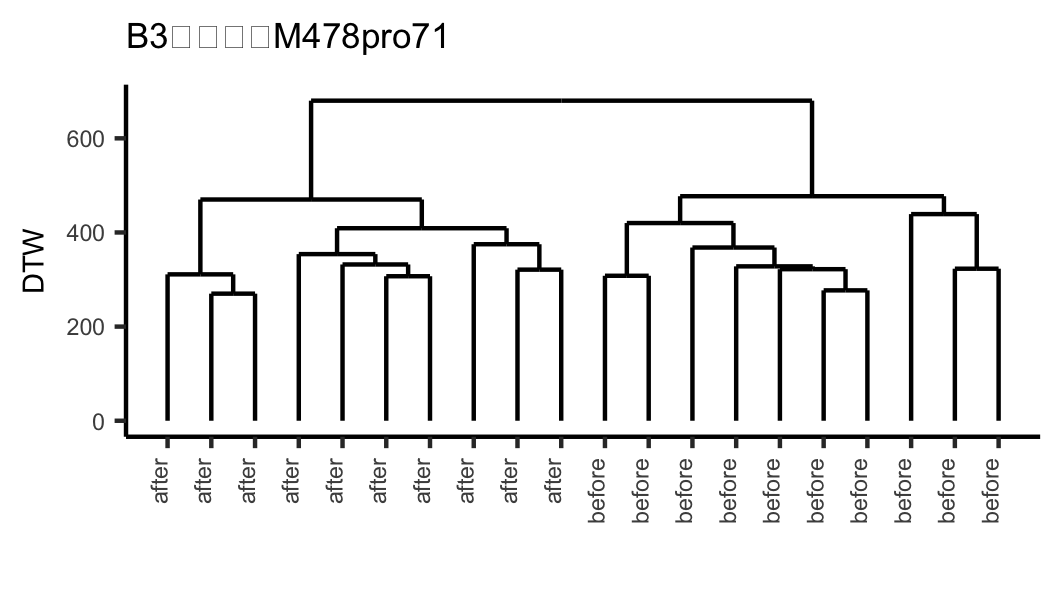
\includegraphics[width=15cm]{fig/dendro_15.png}
		\caption{デンドログラム15}
		\label{fig:dendro15}

	\end{center}
\end{figure}



\section{考察・今後の課題}






\bibliography{TDA} %hoge.bibから拡張子を外した名前


\end{document}